%!TEX root = ../../report.tex
\subsection{Database}
\label{subsec:databaseview}
The figure \ref{fig:database} below shows how the database is structured. Different entities for all types of data are created. This means we store registred citizens, UAV data, sensor data and flood probability. Besides that external data like demographic data and geographical data is stored. The database stores the number of people living in a certain area. Also the altitude of a certain area is stored. This data is used to predict the flood and the potential damage it can cause. To determine the validity, different components are verified. These values are also stored in the database. 

\clearpage
\begin{figure}[H]
	%\centering
	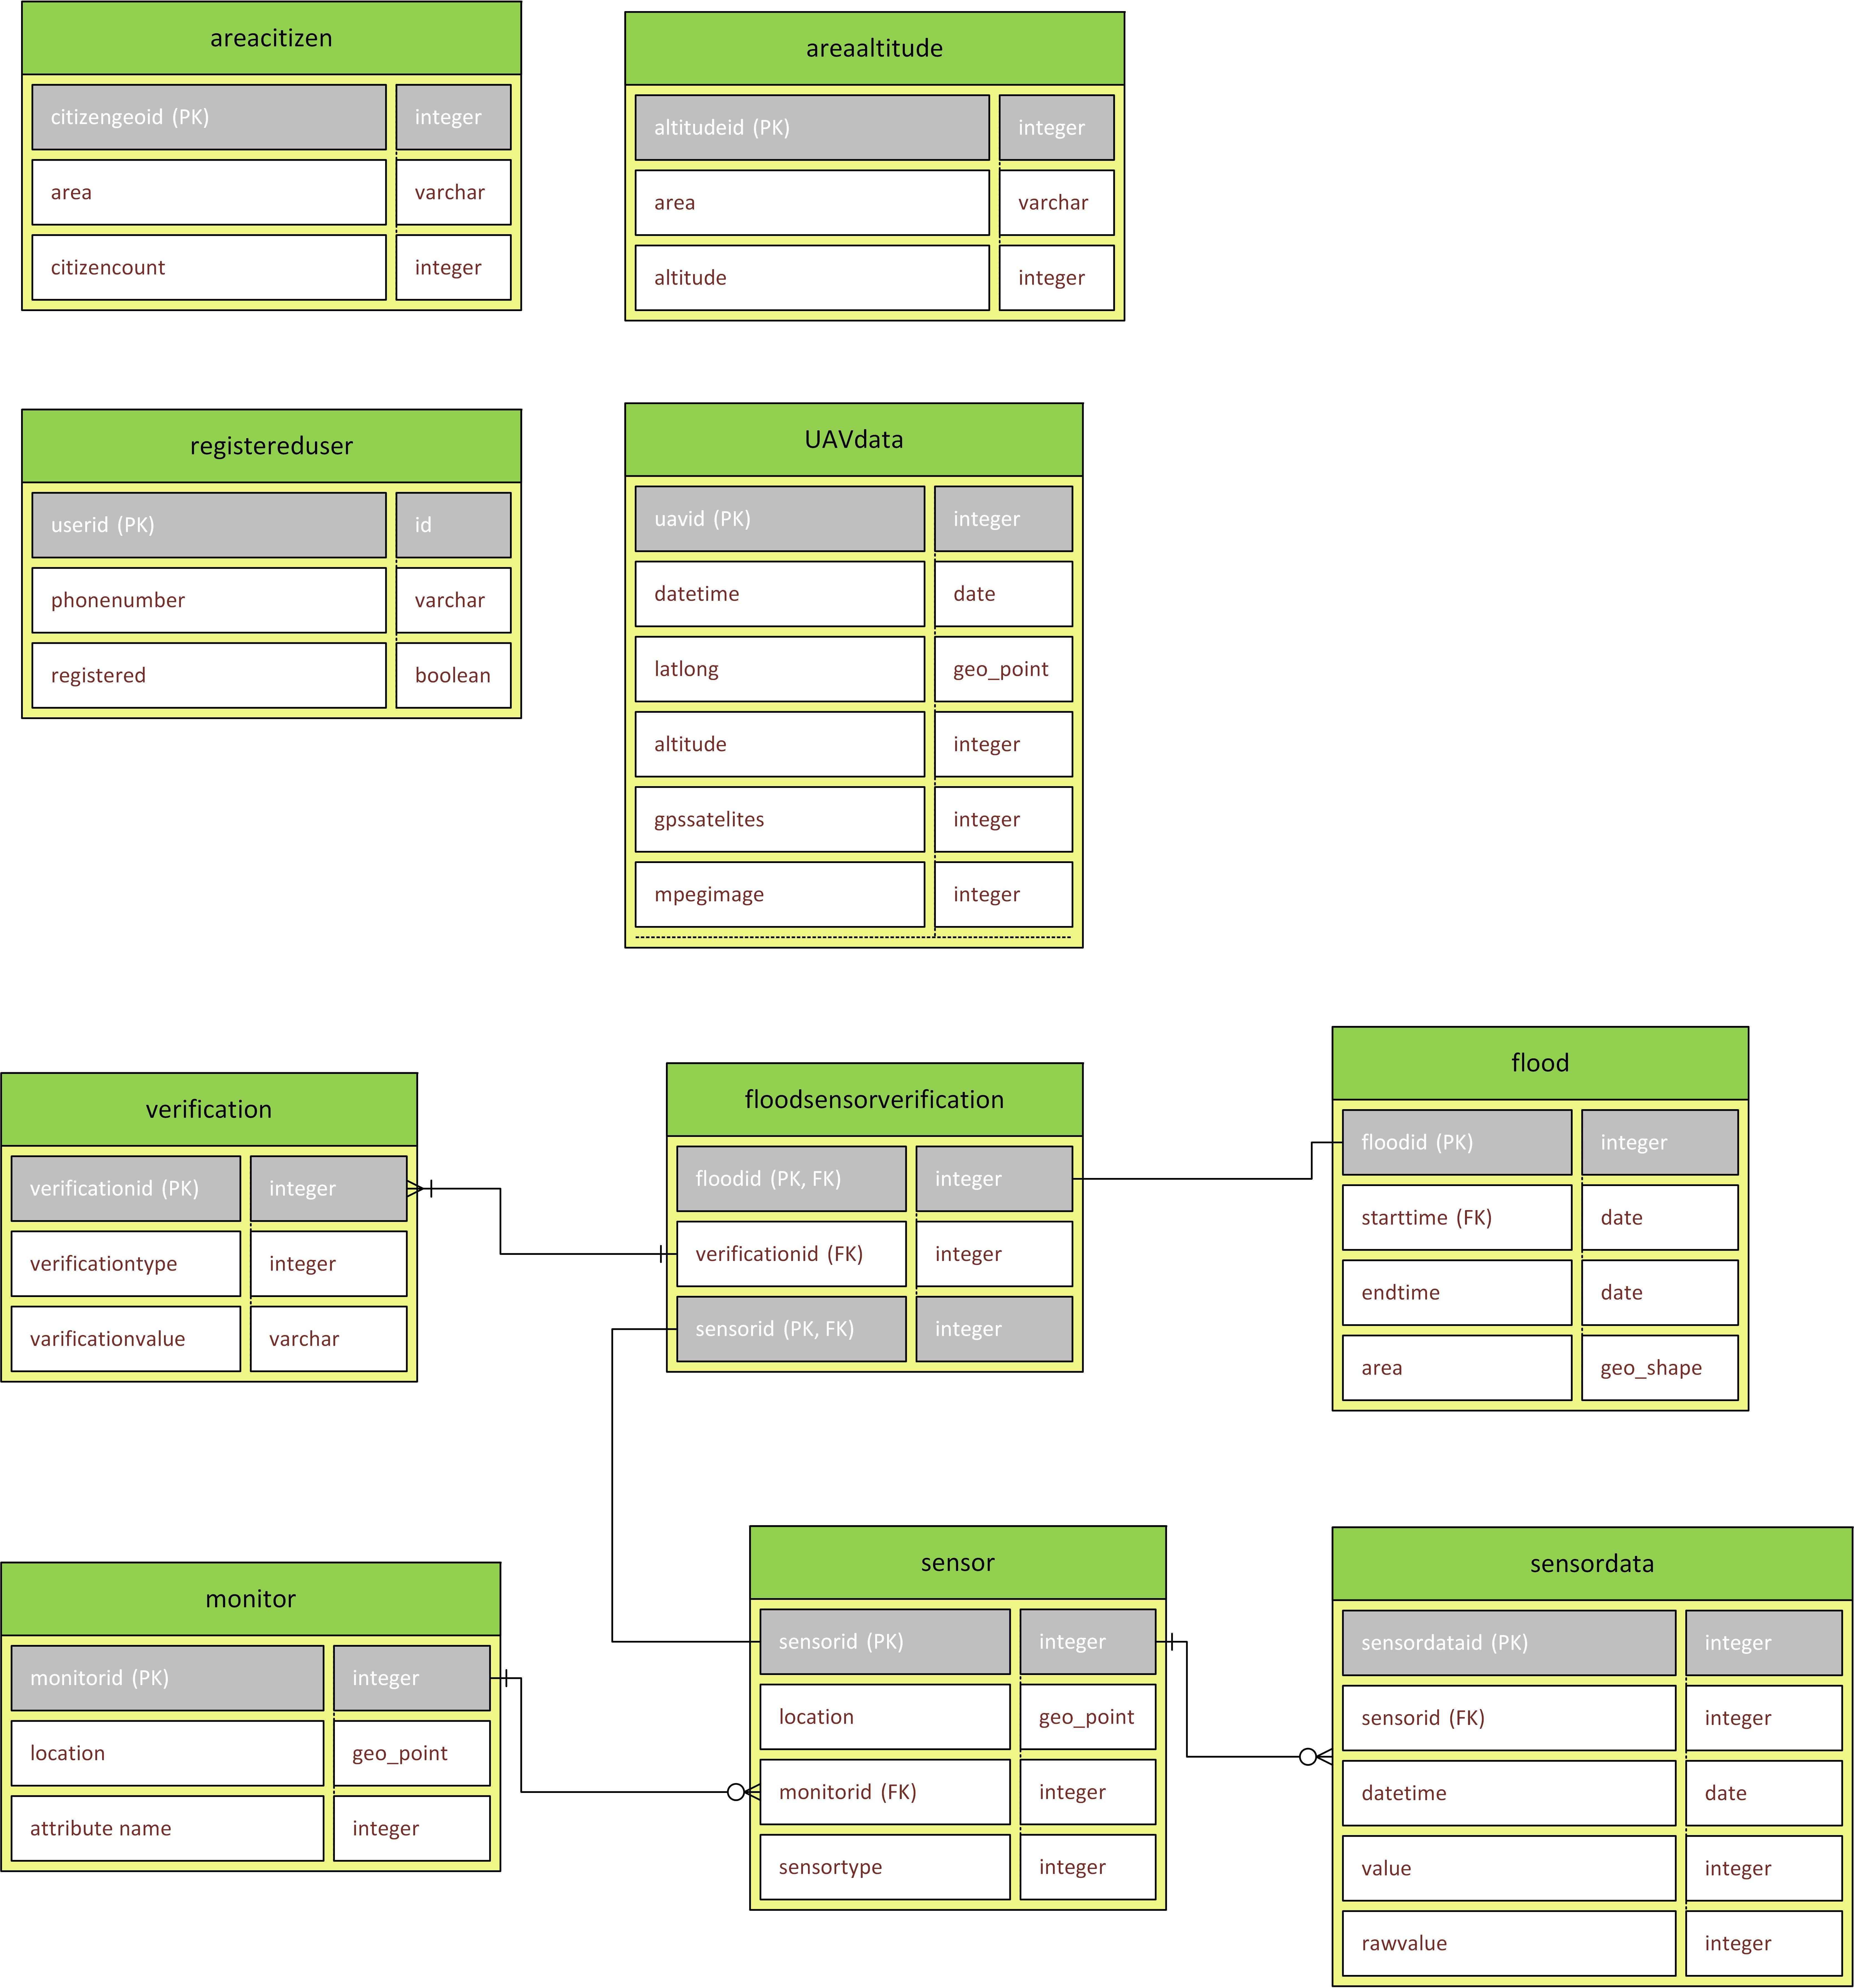
\includegraphics[height=14cm, width=0.9\textwidth]{{\viewimages/database}.jpg}
	\caption{Database diagram}
	\label{fig:database}
\end{figure}





